\section{UML Diagramme}

\begin{bonus}{UML Diagramme}
    \begin{tabular}{|l|l|l|}
        \hline
        \multirow{2}{*}{Strukturdiagramme} & \multicolumn{2}{c|}{Verhaltensdiagramme}                                 \\\cline{2-3}
                                           &                                          & Interaktionsdiagramme         \\\hline
        Klassendiagramm                    & Use-Case-Diagramm                        & Sequenzdiagramm               \\
        Paketdiagramm                      & Aktivitätsdiagramm                       & Kommunikationsdiagramm        \\
        Objektdiagramm                     & Zustandsautomaten                        & Timingdiagramm                \\
        Kompositionsstrukturdiagramm       &                                          & Interaktionsübersichtdiagramm \\
        Komponentendiagramm                &                                          &                               \\
        Verteilungsdiagramm                &                                          &                               \\\hline
    \end{tabular}
\end{bonus}

\subsection{Use-Case-Diagramm}

\begin{defi}{Use-Case-Diagramm}
    \emph{Use-Case-Diagramme} ermöglichen einen einfachen Einstig in die Projektanalyse.
    Des Weiteren zeigen diese das externe Verhalten eines System aus Sicht der Nutzenden, und wie diese mit dem System interagieren um ein Zeil zu erreichen.

    Des weiteren soll das Use-Case Diagramm antworten auf folgende Fragen liefern:
    \begin{itemize}
        \item \emph{Was} soll mein System für seine Umwelt\footnote{Stakeholder, Nachbarsysteme etc.} leisten?
        \item Welche Interaktionsmöglichkeiten zwischen dem System und den Benutzenden sind für ein bestimmtes Ziel definiert.
        \item Durch hohe Kontextabgrenzung entsteht ein hohes Abstraktionsniveau trotz einer einfachen bzw. schlichten Notation.
    \end{itemize}
\end{defi}

\begin{diag}{Use-Case-Diagramm (Aufbau)}
    \begin{center}
        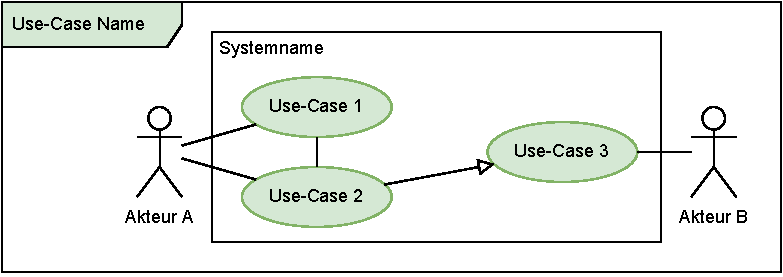
\includegraphics[width=0.75\textwidth]{includes/figures/defi_diagrams_use_case_intro.pdf}
    \end{center}

    Anbei findet man eine tabellarische textuelle Beschreibung jedes relevanten Anwendungsfalls:

    \begin{tabularx}{\textwidth}{|>{\bfseries}l|X|}
        \hline
        \multicolumn{2}{|l|}{Use-Case-Nummer, Use-Case-Name}                                                                                                 \\\hline\hline
        Kurzbeschreibung  & ein kurzer erklärender strukturierter Satz zur Übersicht                                                                         \\\hline
        Akteure           & Personen bzw. Rollen oder externe Systeme, die aktiv mit dem System interagieren oder einen Nutzen von dem Anwendungsfall haben.
        Ein Anwendungsfall kann mit mehreren Akteuren verbunden sein.                                                                                        \\\hline
        Kategorie         & muss, soll oder kann der Anwendungsfall realisiert werden                                                                        \\\hline
        Auslösung         & ein Akteur oder eine Funktion, die den Ablauf startet                                                                            \\\hline
        Vorbedingung      & eine Bedingung, die erfüllt sein muss, damit der Ablauf gestartet wird                                                           \\\hline
        Eingabe / Ausgabe & für den Ablauf benötigte Informationen / Ergebnis des Ablaufs                                                                    \\\hline
        Nachbedingung     & Eine Bedingung, die erfüllt sein muss, um den Anwendungsfall zu beenden                                                          \\\hline
        Ablauf            & beschreibt den Standardablauf - keine Sonderfälle                                                                                \\\hline
    \end{tabularx}
\end{diag}

\begin{diag}{Akteur (Use-Case-Diagramm)}
    \begin{wrapfigure}{r}{0.15\textwidth}
        \centering
        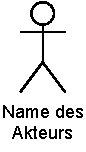
\includegraphics[width=0.1\textwidth]{includes/figures/defi_diagrams_use_case_akteur.pdf}
    \end{wrapfigure}
    %
    Personen oder Rollen werden meist durch \emph{Akteure} beschreiben.

    In Use-Case Diagrammen stoßen diese Akteure Anwendungsfälle an.

    Alternativ stehen neben dem stilisiertem Symbol weitere Rollen-spezifische Symbole zur Verfügung:

    \begin{center}
        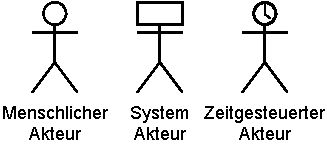
\includegraphics[width=0.4\textwidth]{includes/figures/defi_diagrams_use_case_akteur_types.pdf}
    \end{center}
\end{diag}

\begin{bonus}{Spezifischer Akteur (Use-Case-Diagramm)}
    \begin{wrapfigure}{r}{0.35\textwidth}
        \centering
        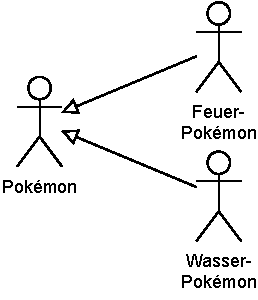
\includegraphics[width=0.3\textwidth]{includes/figures/bonus_diagrams_use_case_akteur_specification.pdf}
    \end{wrapfigure}
    %
    Wenn Akteure durch bestimmte Eigenschaften erweitert werden müssen, jedoch in ihrer Grundform weiterhin benötigt werden, kann man diese \emph{spezifische Rollen} durch allgemeinen Rollen \emph{generalisieren}.

    Dementsprechend wird hier der Akteur \emph{Pokémon} durch \emph{Feuer-} sowie \emph{Wasser-Pokémon} spezialisiert.

    \vspace{7em}
\end{bonus}

\begin{diag}{Use-Case (Use-Case-Diagramm)}
    \begin{wrapfigure}{r}{0.25\textwidth}
        \centering
        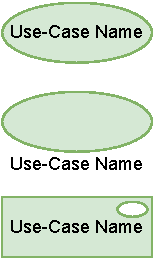
\includegraphics[width=0.2\textwidth]{includes/figures/defi_diagrams_use_case.pdf}
    \end{wrapfigure}
    %
    \emph{Use-Cases} bzw. Anwendungsfälle beschreiben eine Aktivität.
    Dabei besteht der Name aus einem Substantiv und einem Verb.

    Diese werden meist mit einem Oval oder einer Ellipse dargestellt.
    Dabei steht der Name - je nach vorhandenem Platz - entweder in dem Symbol oder darunter.

    \vspace{8em}
\end{diag}

\begin{diag}{Systeme und Grenzen (Use-Case-Diagramm)}
    Um das Gesamtsystem aus fachlicher Sicht einzuordnen, kann man Anwendungsfalls-Gruppen in einem \emph{System} zusammenfügen.
    Diese Systeme grenzen verschiedene fachliche Teile, Aufgaben bzw. Verantwortungsbereiche voneinander ab.

    %Dabei dient die Einteilung nicht als technische Analyse!
\end{diag}

\begin{diag}{Kanten bzw. Assoziationen (Use-Case-Diagramm)}
    \emph{Kanten bzw. Assoziation} modellieren Interaktionen zwischen:
    \begin{itemize}
        \item Akteur und Akteur
        \item Akteur und Use-Case
        \item Use-Case und Use-Case
    \end{itemize}
    und beantworten die Frage, wer mit wem in welcher Beziehung steht.

    Dabei erfolgt die Darstellung über Kanten und Linien, welche ggf. über zusätzliche Annotationen angereichert werden.
\end{diag}

\begin{diag}{Assoziationstypen (Use-Case-Diagramm)}
    \begin{itemize}
        \item \textbf{Binäre Assoziation (ungerichtet)}

              Richtung nicht eindeutig, i.d.R. ausgehend von einem der beteiligten Akteuren

              \vspace{1em}
              \begin{center}
                  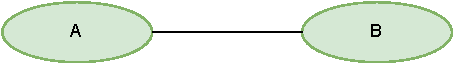
\includegraphics[width=0.5\textwidth]{includes/figures/defi_diagrams_use_case_assoziation.pdf}
              \end{center}

        \item \textbf{Import bzw. Include Beziehung}

              \emph{A} \emph{umfasst} das Verhalten von \emph{B} vollständig.
              D.h. B ist eine Teilfunktion von A.
              A beinhaltet aber noch weitere Teile.
              Dies ist eine klassische Anwendung um Redundanzen zu vermeiden:
              Mehrere Use-Cases führen denselben Teil aus, dann wird er ausgelagert und gemeinsam genutzt.

              \vspace{1em}
              \begin{center}
                  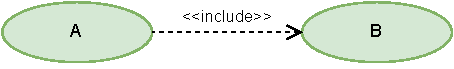
\includegraphics[width=0.5\textwidth]{includes/figures/defi_diagrams_use_case_include.pdf}
              \end{center}

        \item \textbf{Erweiterungsbeziehung}

              \emph{A} \emph{erweitert} \emph{B} unter einer speziellen Voraussetzung

              \vspace{1em}
              \begin{center}
                  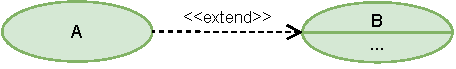
\includegraphics[width=0.5\textwidth]{includes/figures/defi_diagrams_use_case_extend.pdf}
              \end{center}

        \item \textbf{Generalisierungsbeziehung}

              \emph{A} ist ein \emph{B}.
              Interessant bei abstrakten Akteuren und / oder Teilsystemen.

              \vspace{1em}
              \begin{center}
                  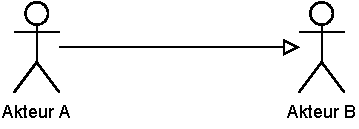
\includegraphics[width=0.4\textwidth]{includes/figures/defi_diagrams_use_case_generalisierung.pdf}
              \end{center}
    \end{itemize}

    Obacht: Bei der Angabe mehrerer Assoziationen ist die Reihenfolge nicht festgelegt.
\end{diag}

\begin{example}{Use-Case-Diagramm}
    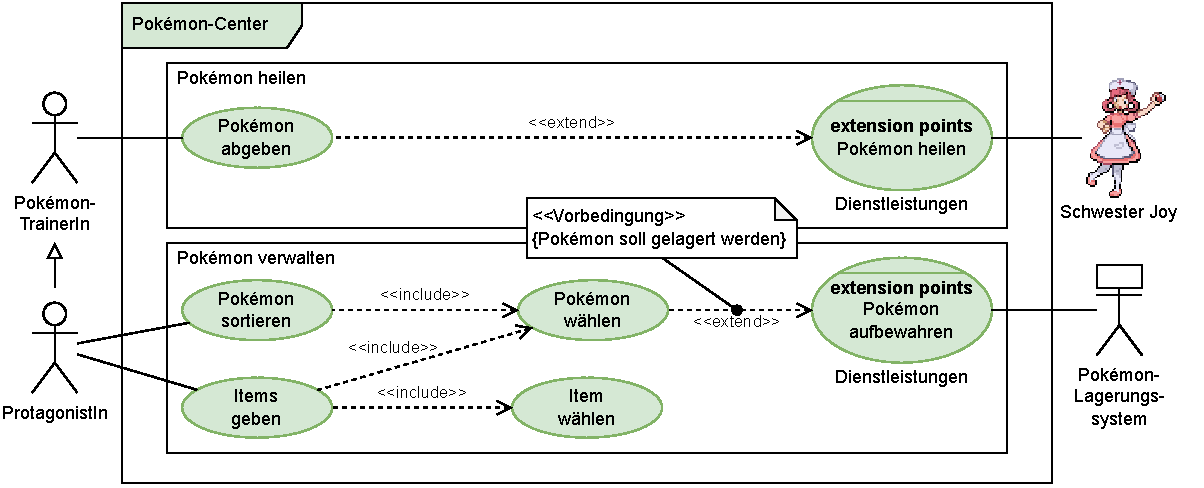
\includegraphics[width=\textwidth]{includes/figures/example_diagrams_use_case.pdf}
\end{example}

\begin{example}{Use-Case-Diagramm (Textuelle Beschreibung)}
    \begin{tabularx}{\textwidth}{|>{\bfseries}l|X|}
        \hline
        \multicolumn{2}{|l|}{UC2: Pokémon sortieren}                                                                           \\\hline\hline
        Kurzbeschreibung  & Verwaltet das aktuelle Team und tauscht - falls nötig - Pokémon aus dem Pokémon-Lagerungsystem ein \\\hline
        Akteure           & ProtagonistIn                                                                                      \\\hline
        Kategorie         & kann                                                                                               \\\hline
        Auslösung         & Entscheidung das Team zu modifizieren                                                              \\\hline
        Vorbedingung      & mind. zwei Pokémon im Team bzw. in der Box vorhanden                                               \\\hline
        Eingabe / Ausgabe & E: Altes Team, Modifikation, A: Neues Team                                                         \\\hline
        Nachbedingung     & Pokémon wurden gewählt und getauscht                                                               \\\hline
        Ablauf            & \begin{enumerate}
            \item ProtagonistIn betritt das Pokémon-Center
            \item ProtagonistIn meldet sich am Pokémon-Lagerungsystem an
            \item Solange ProtagonistIn nicht fertig
                  \begin{enumerate}
                      \item Wähle auszutauschendes Pokémon
                      \item Wähle einzutauschendes Pokémon
                  \end{enumerate}
        \end{enumerate}                                                                        \\\hline
    \end{tabularx}
\end{example}

\subsection{Aktivitätsdiagramm}

\begin{defi}{Aktivitätsdiagramm}
    Primär beantworten \emph{Aktivitätsdiagramme} die Frage, \emph{wie} eine Aktivität realisiert werden soll.
    Sie stellen konkrete komplexe Abläufe dar, indem sie diese wie folgt zerlegen:
    \begin{itemize}
        \item Nebenläufe
        \item alternative Entscheidungswege
        \item Einzelschritte von Aufgaben
    \end{itemize}

    Aktivitätsdiagramme können für folgende Objekte genutzt werden:
    \begin{itemize}
        \item einen Use-Case
        \item eine Operation
        \item ein Geschäftsmodell
    \end{itemize}
\end{defi}

\begin{diag}{Aktivitätsdiagramm (Aufbau)}
    \begin{center}
        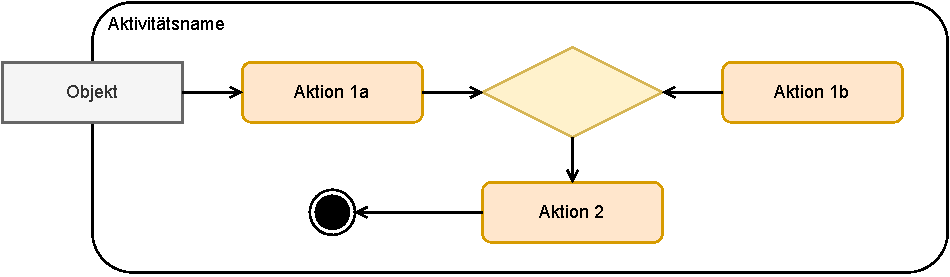
\includegraphics[width=0.75\textwidth]{includes/figures/defi_diagrams_activity_intro.pdf}
    \end{center}
\end{diag}

\begin{diag}{Aktion (Aktivitätsdiagramm)}
    \begin{wrapfigure}{r}{0.25\textwidth}
        \centering
        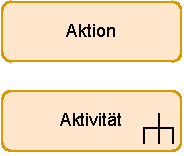
\includegraphics[width=0.2\textwidth]{includes/figures/defi_diagrams_activity_aktion.pdf}
    \end{wrapfigure}
    %
    Eine \emph{Aktion} ist ein Einzelschritt, den ein Ablauf unter Zeitaufwand durchschreitet.

    Aktionen können in einem Aktivitätsdiagramm eine weitere Aktivität aufrufen.
    Dies kennzeichnet man durch eine \enquote{stilisierte Harke}.

    In diesen Unteraktivitäten können Eingangs- sowie Ausgangsparameter durch Objektknoten festgelegt werden.
\end{diag}

\begin{diag}{Objektknoten (Aktivitätsdiagramm)}
    \begin{wrapfigure}{r}{0.25\textwidth}
        \centering
        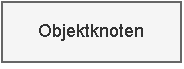
\includegraphics[width=0.2\textwidth]{includes/figures/defi_diagrams_activity_objektknoten.pdf}
    \end{wrapfigure}
    %
    \emph{Objektknoten} beinhalten beteiligte Daten und dienen als Schnittstelle für eine Aktion.

    Bei Unterdiagrammen können Objektknoten als Eingangsparameter die Unteraktivität starten.

    Beim Übergeben von Objektknoten zwischen Aktionen, werden die Objekte als kleines Rechteck vor bzw. hinter der Aktion dargestellt.
\end{diag}

\begin{diag}{Kontrollelemente zur Ablaufsteuerung (Aktivitätsdiagramm)}
    \begin{wrapfigure}{r}{0.25\textwidth}
        \centering
        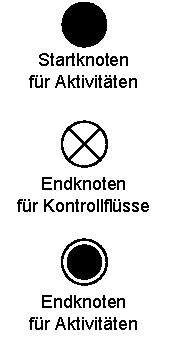
\includegraphics[width=0.175\textwidth]{includes/figures/defi_diagrams_activity_start_end.pdf}
    \end{wrapfigure}
    \textbf{Startknoten}:
    \begin{itemize}
        \item Markiert den Startpunkt eines Ablaufs beim Aktivieren einer Aktivität
        \item Eine Aktivität kann beliebig viele Startknoten haben (Nebenläufige Ausführung an allen Startknoten)
        \item Eine Aktivität muss keinen Startknoten besitzen (Eingabeparameter dienen als Startpunkt)
        \item Jeder Startknoten erstellt ein Token, welches der anliegenden Kante mitgegeben wird.
    \end{itemize}

    \textbf{Endknoten für Kontrollflüsse}:
    \begin{itemize}
        \item Beendet nur einen einzelnen Ablauf, indem das aktuell anliegende Token gelöscht wird.
        \item Nebenläufig ausgeführte Aktionen werden nicht beendet.
        \item Beendigung der gesamten Aktivität daher nur bei nicht parallelisierten Abläufen
    \end{itemize}

    \textbf{Endknoten für Aktivitäten}:
    \begin{itemize}
        \item Beendet sofort die gesamte Aktivität, indem alle Tokens gelöscht werden.
        \item Parallel ausgeführte Aktionen werden ebenfalls beendet
    \end{itemize}
\end{diag}

\begin{diag}{Kontrollelemente zur Ablaufsteuerung für Bedingungen (Aktivitätsdiagramm)}
    \begin{wrapfigure}{r}{0.25\textwidth}
        \centering
        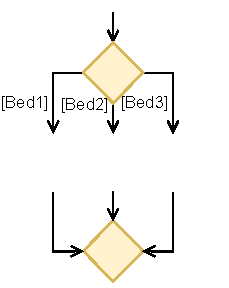
\includegraphics[width=0.2\textwidth]{includes/figures/defi_diagrams_activity_or.pdf}
    \end{wrapfigure}
    \textbf{Verzweigungsknoten}:
    \begin{itemize}
        \item Spaltet eine Kante in mehrere Alternativen auf.
              Dabei kann der Verzweigungsknoten \emph{maximal einen} Token weitergeben.
        \item Programmfluss wird von Bedingungen abhängig gemacht.
        \item Bei mehreren ausgehenden Kanten müssen alle Bedingungen disjunkt sein.
    \end{itemize}

    \textbf{Verbindungsknoten}:
    \begin{itemize}
        \item Führt mehrere unabhängige Kanten in einem gemeinsamen Programmfluss zusammen.
              Dabei ist es egal, wie viele Token aus welchen Kanten ankommen - jedes Token wird von dem Verbindungsknoten direkt weitergeleitet.
    \end{itemize}
\end{diag}

\begin{diag}{Kontrollelemente zur Ablaufsteuerung zur Parallelisierung (Aktivitätsdiagramm)}
    \begin{wrapfigure}{r}{0.25\textwidth}
        \centering
        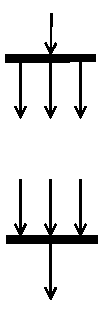
\includegraphics[width=0.1\textwidth]{includes/figures/defi_diagrams_activity_and.pdf}
    \end{wrapfigure}
    \textbf{Parallelisierungsknoten}:
    \begin{itemize}
        \item Teilt den Ablauf einer eingehenden Kante in mehrere parallele Abläufe auf.
              Dabei muss der Parallelisierungsknoten \emph{exakt so viele} Tokens weitergeben, wie ausgehenden Kanten vorhanden sind.
        \item Ermöglicht Nebenläufigkeit von Aktionen.
        \item Kontroll- bzw. Objektfluss muss am Ende wieder zusammengefasst oder getrennt werden.
    \end{itemize}

    \textbf{Synchronisationsknoten}:
    \begin{itemize}
        \item Vereint parallele Abläufe.
              Dabei muss aus jeder eingehenden Kante \emph{mindestens ein} Token empfangen werden.
              Diese werden im Anschluss gebündelt weitergeleitet.
    \end{itemize}
\end{diag}

\begin{diag}{Signale und Ereignisse zur Parallelisierung (Aktivitätsdiagramm)}
    \begin{wrapfigure}{r}{0.25\textwidth}
        \centering
        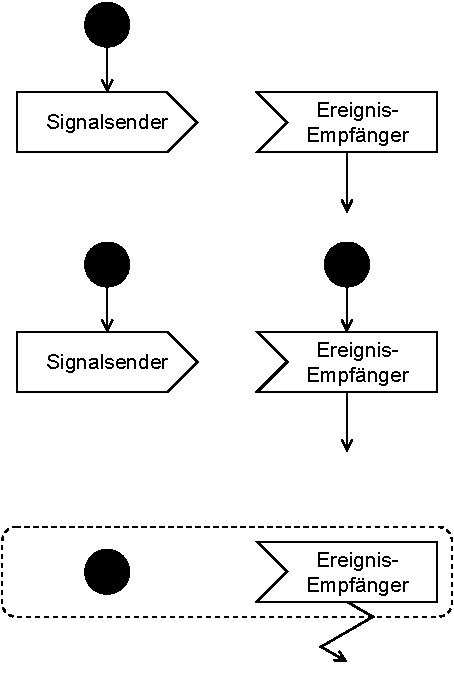
\includegraphics[width=0.25\textwidth]{includes/figures/defi_diagrams_activity_signal.pdf}
    \end{wrapfigure}
    \textbf{Signal Sender}:
    \begin{itemize}
        \item Löst die Sonderaktion \emph{SendSiganlAction} aus, sobald ein Token das Objekt erreicht.
    \end{itemize}

    \textbf{Ereignisempfänger}:
    \begin{itemize}
        \item Löst die Sonderaktion \emph{AcceptEventAction} aus, sobald ein Signal gesendet wurde.
        \item Diese Objekte erscheinen in drei Variationen:
              \begin{itemize}
                  \item Ereignisempfänger \emph{ohne einlaufende Kante}

                        Dieser reagiert unmittelbar nach Erhalt des Sendesignals wie eine normale Aktion.
                  \item Ereignisempfänger \emph{mit einlaufender Kante}

                        Dieser reagiert erst, wenn sowohl ein Sendesignal empfangen wurde, als auch ein Token durch die anliegende Kante erhalten wurde.
                  \item Ereignisempfänger \emph{mit Unterbrechungskante}

                        Dieser reagiert unmittelbar nach Erhalt des Sendesignals.
                        Zusätzlich wird der Gruppierungsbereich\footnote{Anliegende gestrichelte Linie} unterbrochen, und der Programmfluss wird am Ende der anliegenden Unterbrechungskante fortgesetzt.
              \end{itemize}
    \end{itemize}
\end{diag}

\subsection{Klassendiagramm}

\begin{defi}{Klassendiagramm}
    \emph{Klassendiagramme} existieren in zwei verschiedenen Formen:

    \begin{itemize}
        \item \textbf{Klassendiagramm für Analysemodell}
              \begin{itemize}
                  \item Klassen mit Attributen
                  \item Assoziationen, Vererbung,  Multiplizitäten
                  \item Kompositionen, Aggregationen
              \end{itemize}
        \item \textbf{Klassendiagramm für Entwurfsmodell} (erweitert das Analysemodell)
              \begin{itemize}
                  \item Operationen bzw. Methoden, Funktionen
                  \item Klassen- und Objekteigenschaften
                  \item Abgeleitete Eigenschaften, Sichtbarkeiten
                  \item Navigationsrichtungen
                  \item Eigenschaften von Attributen und Assoziationsenden
                  \item Qualifizierte Assoziationen
                  \item Klassenarten
                  \item Abhängigkeiten
              \end{itemize}
    \end{itemize}

    Sie liefern eine Antwort auf die Frage:
    \begin{itemize}
        \item \emph{Welche} Datentypen werden in dem System genutzt?
        \item \emph{Wie} verhalten sich diese Objekte im Detail?
    \end{itemize}
\end{defi}

% \begin{defi}{Klassendiagramm (Aufbau)}
%     \begin{center}
%         \includegraphics[width=0.35\textwidth]{includes/figures/03_class_diagram.pdf}
%     \end{center}
% \end{defi}

\begin{diag}{Klasse (Klassendiagramm)}
    \begin{wrapfigure}{r}{0.25\textwidth}
        \centering
        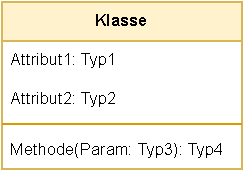
\includegraphics[width=0.25\textwidth]{includes/figures/defi_diagrams_class_intro.pdf}
    \end{wrapfigure}
    %
    UML \emph{Klassen} entsprechen den programmatischen Klassen aus bekannten objektorientierten Sprachen.

    Das Symbol besteht aus einem Header mit dem großgeschriebenen, fettgedruckten, horizontal mittig zentrierten Klassennamen und zwei \enquote{Containern}.
    Diese werden mit potentiellen Attributen (oben) und Operationen bzw. Methoden (unten) der Klasse gefüllt.

    Hier werden einige weitere Symbole bzw. Schlüsselworte benötigt\footnote{default ist \texttt{\textasciitilde \ \{unordered, unique\}}}:
    \begin{itemize}
        \item Sichtbarkeit:
              \subitem + : \texttt{public}
              \subitem - : \texttt{private}
              \subitem \# : \texttt{protected}
              \subitem \textasciitilde\ : \texttt{package}
              \subitem / : Abgeleitetes Attribut
        \item \texttt{\{id\}}: Attribut entspricht einem Primärschlüssel
        \item \texttt{\{readOnly\}}
        \item \texttt{\{frozen\}} bzw. \texttt{\{immutable\}}
        \item \texttt{\{abstract\}}\footnote{alternativ kann man das jeweilige Objekt in kursiv schreiben}
        \item \texttt{static}: Das jeweilige Objekt muss unterstrichen sein
        \item \texttt{generic} bzw Parametrisiert : Die Klasse wird mit einem kleinen Kasten gekennzeichnet, indem alle generischen Typen zu finden sind.
        \item Kollektionen
              \subitem \texttt{\{ordered\}} oder \texttt{\{unordered\}}
              \subitem \texttt{\{unique\}} oder \texttt{\{nonunique\}}
        \item \texttt{<<interface>>}
        \item \texttt{<<utility>>}: Hilfsklassen (diese werden via \texttt{<<use>> genutzt})
    \end{itemize}
\end{diag}

\begin{diag}{Attribut (Klassendiagramm)}
    Jedes \emph{Attribut} benötigt eine Typangabe\footnote{Man achte auf die exakte Schreibweise; (Primitive-) Datentypen werden groß- und ausgeschrieben}.

    Der Typ wird nach dem kleingeschriebenen Attributnamen mit einem \texttt{:} angegeben.

    Attribute, welche als Fremdschlüssel für andere Klassen dienen, können ebenfalls aufgeführt werden.
    Alternativ schreibt man die Bezeichnung an die Assoziation.\footnote{Siehe Navigierbarkeit, Erreichbarkeit}

    Multiplizitäten für Kollektionen:

    \begin{tabular}{>{\ttfamily}l>{\ttfamily}lll}
        \multicolumn{1}{l}{Symbol} & \multicolumn{1}{l}{alternativ} & Typ          & {Multiplizität}                       \\
        \hline
        $[$n..m$]$                 &                                &              & zwischen mindestens n und höchstens m \\
        $[$0..1$]$                 & $[$1$]$                        & optional     & höchstens ein Wert                    \\
        $[$0..*$]$                 & $[$*$]$                        & optional     & beliebig viele Werte                  \\
        $[$1..*$]$                 &                                & erforderlich & beliebig viele Werte
    \end{tabular}
\end{diag}

\begin{diag}{Operation (Klassendiagramm)}
    Unter \emph{Operationen} fallen alle klassenabhängigen Methoden und Funktionen.

    Parametrisierte Konstruktoren müssen dort wie gewöhnliche Operationen aufgeführt werden.

    Eine Operation beinhaltet einen Namen, eine Parameterliste und einen Rückgabetyp.
    Diese folgen folgender Syntax:

    \begin{center}
        \texttt{<Name> ( <Parameterliste> ) [: <Rückgabetyp>]}
    \end{center}

    Die Parameterliste ist eine durch Kommata getrennte Aufzählung von Parametern.
    Parameter werden wie folgt dargestellt:

    \begin{center}
        \texttt{[Richtung] <Name> : <Typ> [Multiplizität][Standardwert]}
    \end{center}

    Unter Richtungen fallen:
    \begin{itemize}
        \item \texttt{in}: Call-by-Value
        \item \texttt{inout}: Call-by-Reference
        \item \texttt{out}: initialisiert den Out-Parameter beim Aufrufen der Operation und stellt diesen in dem Scope, in dem die Operation aufgerufen wurde, zur Verfügung.
    \end{itemize}
\end{diag}

\begin{diag}{Assoziation}
    Eine \emph{Assoziation} ist dann navigierbar, wenn Objekte der adjazenten Klasse erreichbar sind.

    \begin{wrapfigure}{r}{0.25\textwidth}
        \centering
        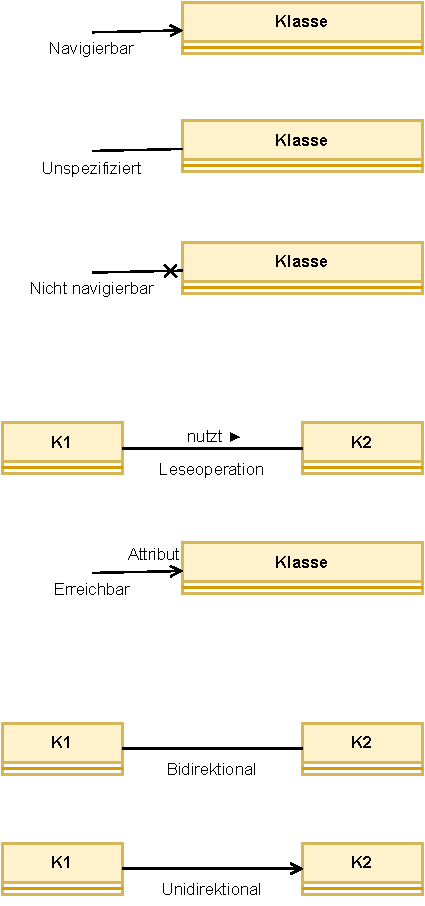
\includegraphics[width=0.25\textwidth]{includes/figures/defi_diagrams_class_assoziation.pdf}
    \end{wrapfigure}
    \textbf{Navigierbarkeit}:

    Dabei hat jede Assoziation eine von drei möglichen Navigationszuständen:
    \begin{itemize}
        \item navigierbar
        \item unspezifiziert
        \item nicht navigierbar
    \end{itemize}

    \textbf{Erreichbarkeit}:

    Sollte die Klasse erreichbar sein, muss man eine Leseoperation zur Verfügung stellen.
    Des Weiteren muss man sich überlegen, wie man das Objekt erreichen kann:
    \begin{itemize}
        \item Als Attribut in einer Klasse (siehe rechts)
        \item In Datencontainern, wie \texttt{Hashtables}
        \item \ldots
    \end{itemize}

    \textbf{Erreichbarkeitsrichtung}:

    Man unterscheidet Assoziationen wie folgt:
    \begin{itemize}
        \item Bidirektional: Beide Klassen sind untereinander erreichbar
        \item Unidirektional: Ausschließlich eine Klasse ist erreichbar
    \end{itemize}
\end{diag}

\begin{diag}{Generalisierung}
    \begin{wrapfigure}{r}{0.25\textwidth}
        \centering
        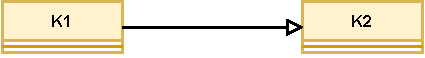
\includegraphics[width=0.25\textwidth]{includes/figures/defi_diagrams_class_vererbung.pdf}
    \end{wrapfigure}
    %
    Eine \emph{Generalisierung} in der UML ist eine gerichtete Beziehung zwischen einer speziellen und einer genereller Klasse.

    Instanzen der speziellen Klasse sind damit auch Instanzen der generellen Klasse.

    Die Klasse \emph{K1} \emph{erbt} z.B. von der Klasse \emph{K2}.
\end{diag}

\begin{diag}{Aggregation und Komposition}
    \begin{wrapfigure}{r}{0.25\textwidth}
        \centering
        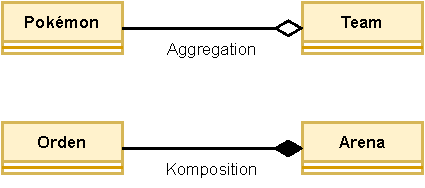
\includegraphics[width=0.25\textwidth]{includes/figures/defi_diagrams_class_aggregation_composition.pdf}
    \end{wrapfigure}
    %
    Zwei Spezialfälle der Assoziation bilden eine Teil-Ganzes-Beziehung.

    \begin{itemize}
        \item \textbf{Aggregation}:

              Ein Objekt (Aggregat) besteht aus mehreren Einzelobjekten.
              Die Lebensdauer der Einzelobjekte kann länger sein als die des Aggregats.
        \item \textbf{Komposition} bzw. Aggregationskomposition:

              Das Teilobjekt ist von der Existenz des Ganzen abhängig.
              Es kann nicht ohne existieren.
    \end{itemize}
\end{diag}

\begin{diag}{Pakete}
    \begin{wrapfigure}{r}{0.25\textwidth}
        \centering
        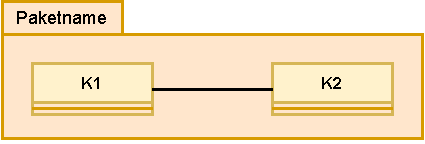
\includegraphics[width=0.25\textwidth]{includes/figures/defi_diagrams_class_package.pdf}
    \end{wrapfigure}
    %
    In der UML dienen \emph{Pakete} zur hierarchisch geschachtelten Strukturierung großer Modelle.
    Jedes Modellelement gehört zu höchstens einem Paket, kann jedoch in mehreren Modellen vorkommen.

    So kann man eine angemessen große Menge modular zerlegter Objekte zu einer logisch geschlossenen Einheit zusammenfassen, welche in größeren Diagrammen genutzt wird.

    Pakete verfolgen das Prinzip der \emph{hohen Kohäsion} und \emph{losen Kopplung}.
\end{diag}

\begin{defi}{Kohäsion}
    \emph{Kohäsion} beschreibt die Kräfte, die ein Modul im Inneren zusammenhalten.

    Eine gewollte starke Kohäsion bedeutet, dass die Teile des Moduls bzw. Pakets eng Zusammenhängen.
    Also werden logische Zusammenhänge ebenfalls strukturell verbunden.
\end{defi}

\begin{defi}{Kopplung}
    \emph{Kopplung} beschreibt die Bindungen, die verschiedene Pakete zusammenhalten.

    Eine gewollte lose (Daten-) Kopplung bewirkt, dass die Module nicht wissen, welche Daten in anderen Modulen gespeichert bzw. berechnet werden.
    Dies wird \emph{Information Hiding} genannt.

    Eine strikte Trennung von Paketen nach dem Prinzip der hohen Kohäsion bewirkt ebenfalls eine lose Kopplung.
    Analog bewirkt lose Kohäsion eine starke Bindung.
\end{defi}

\begin{example}{Kohäsion und Kopplung}
    \begin{wrapfigure}{r}{0.25\textwidth}
        \centering
        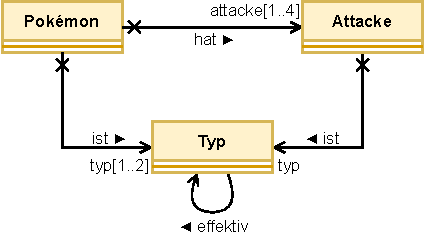
\includegraphics[width=0.25\textwidth]{includes/figures/example_diagrams_class_kohaesion.pdf}
    \end{wrapfigure}
    Beispiel für gewollte starke (funktionale) Kohäsion:
    \begin{itemize}
        \item Die Klassen Pokémon, Typ, Attacke
              \begin{itemize}
                  \item Jedes Pokémon hat mindestens einen Typen.
                  \item Jedes Pokémon hat zusätzlich bis zu vier Attacken.
                  \item Jede Attacke hat ebenfalls einen Typen.
                  \item Jeder Typ ist effektiv gegen andere Typen.
              \end{itemize}

              Wenn man nun eine Klasse aus dem Paket entnimmt und zu einem eigenen Paket macht, erstellt man automatisch 2 Verbindungen zwischen dem aktuellen und dem neuen Paket.
              Da dies eine surjektive Assoziation wäre\footnote{Jedes Element der Zielmenge wird getroffen}, ist hier ein Aufteilen nicht sinnvoll.
    \end{itemize}

    Beispiel für schwache (zufällige) Kohäsion:
    \begin{itemize}
        \item \texttt{getter-}, \texttt{setter-} sowie \texttt{print-} Methoden speichern die Daten des jeweiligen Objekts nicht.
              Dementsprechend kann man diese Methoden im Modell von dem Objekt trennen.
        \item Die Assoziation zwischen Arena bzw. Orden mit der / dem ProtagonistIn.
              \begin{itemize}
                  \item Jede/r ProtagonistIn kann beliebig viele Orden in Arenen freischalten.

                        Hier ist eine Abtrennung eines Arena/Orden-Pakets möglich.
                  \item zwischen Arena und Orden liegt ein hohes Maß an Kohäsion vor.

                        Hier ist eine weitere Trennung nicht sinnvoll.
              \end{itemize}
    \end{itemize}
\end{example}

\subsection{Sequenzdiagramm}

\begin{defi}{Sequenzdiagramm}
    \emph{Sequenzdiagramme} zeigen den Informationsaustausch via Nachrichten von Kommunikationspartnern zwischen Systemen oder innerhalb eines Systems für \emph{ein} konkretes Szenario.

    Sie liefern Antworten auf die Frage:
    \emph{Wie} läuft die Kommunikation in meinem System ab?
\end{defi}

\begin{diag}{Sequenzdiagramm (Aufbau)}
    \begin{center}
        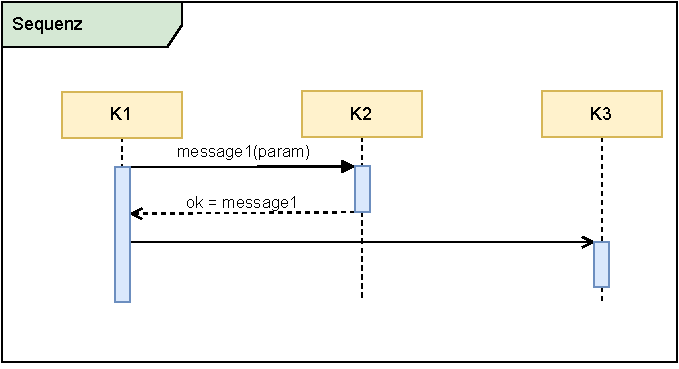
\includegraphics[width=0.75\textwidth]{includes/figures/defi_diagrams_sequenz_intro.pdf}
    \end{center}
\end{diag}

\begin{diag}{Interaktion}
    Eine \emph{Interaktion} verbindet mehrere kommunizierende Objekte und regelt den Kommunikationsfluss mithilfe ausgetauschter Nachrichten.

    Die beteiligten Objekte treten paarweise in den Rollen Sender und Empfänger auf.
\end{diag}

\begin{diag}{Lebenslinien (Sequenzdiagramm)}
    \begin{wrapfigure}{r}{0.25\textwidth}
        \centering
        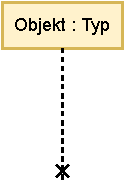
\includegraphics[width=0.2\textwidth]{includes/figures/defi_diagrams_sequenz_object.pdf}
    \end{wrapfigure}
    %
    \emph{Lebenslinien} repräsentieren genau eine teilnehmende Objektinstanz\footnote{Klassen können ebenfalls in verschiedene Lebenslinien für strikt getrennte Operationsbereiche getrennt werden.}.
    Sie verdeutlichen einen spezifischen zeitlichen Ablauf.

    Ein Kommunikationspartner lebt bis ans Ende des Diagramms oder bis zum expliziten Beenden der Lebenslinie durch ein \enquote{x}.

    Es existieren 3 verschiedene Typen von Objektarten:
    \begin{itemize}
        \item \emph{Expliziter Name ohne Typangabe}:

              Gilt für eine feste Instanz, dessen Identität bekannt ist.
        \item \emph{Expliziter Name mit Typangabe}:

              Gilt für eine feste Instanz, dessen Identität und exakter Typ bekannt ist.
        \item \emph{Anonyme Instanz mit Typangabe}:

              Gilt für eine feste aber beliebige Instanz des angegebenen Typen, dessen Identität noch nicht bekannt ist.
    \end{itemize}
\end{diag}

\begin{diag}{Aktionssequenzen bzw. Aktivierungsbalken (Sequenzdiagramm)}
    \begin{wrapfigure}{r}{0.25\textwidth}
        \centering
        
\includegraphics[width=0.025\textwidth]{includes/figures/defi_diagrams_sequenz_aktion.pdf}
    \end{wrapfigure}
    %
    \emph{Aktionssequenzen} bzw. \emph{Aktivierungsbalken} verdeutlichen einen Kommunikationsfluss.
    Sie sind keine Pflicht, jedoch hilfreich.

    Innerhalb dieser Aktivierungsbalken können beispielsweise Operationen bzw. Methoden der Instanz aufgerufen, oder eine Interaktion gestartet werden.

    \vspace{1cm}
\end{diag}

\begin{diag}{Nachricht (Sequenzdiagramm)}
    \begin{wrapfigure}{r}{0.25\textwidth}
        \centering
        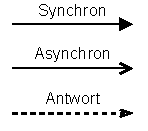
\includegraphics[width=0.2\textwidth]{includes/figures/defi_diagrams_sequenz_message.pdf}
    \end{wrapfigure}
    %
    Die UML unterscheidet bei \emph{Nachrichten} zwischen asynchroner und synchroner Kommunikation:
    \begin{itemize}
        \item \textbf{Synchrone Kommunikation}:
              \begin{enumerate}
                  \item Sender versendet synchrone Nachricht und blockiert.
                  \item Empfänger verarbeitet die Nachricht.
                  \item Empfänger liefert eine Antwort.
                  \item Sender empfängt Antwortnachricht und löst Blockade.
                  \item Sender fährt mit der Bearbeitung seiner Lebenslinie fort.
              \end{enumerate}
        \item \textbf{Asynchrone Kommunikation}:
              \begin{enumerate}
                  \item Sender verschickt Asynchrone Nachricht.
                  \item Sender fährt mit der Bearbeitung seiner Lebenslinie fort\footnote{
                            Im Gegensatz zu der synchronen Kommunikation sperrt der Sender nach der ersten Nachricht nicht.
                            Er führt die Bearbeitung parallel nebenbei fort.
                            Dies passiert bei der synchronen Variante erst bei Schritt 5
                        }.
                  \item Gleichzeitig verarbeitet der Empfänger die Nachricht.
                  \item Empfänger liefert eine Antwort\footnote{Diese ist meist ebenfalls asynchron}.
              \end{enumerate}
    \end{itemize}

    Es ist ebenfalls möglich, dass Instanzen Nachrichten an sich selber senden.
    Diese Starten einen neuen Aktionsbalken in dem aktuellen Aktionsbalken.

    \begin{wrapfigure}{r}{0.35\textwidth}
        \centering
        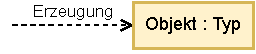
\includegraphics[width=0.3\textwidth]{includes/figures/defi_diagrams_sequenz_message_create.pdf}
    \end{wrapfigure}
    %
    \textbf{Nachricht als Konstruktoraufruf}:

    Alternativ kann man ebenfalls ein neues Objekt mit einer Nachricht erstellen.
    Als Nachrichtenparameter dienen hierbei die für den Konstruktor relevanten Attribute.

    Dabei stehen einem natürlich alle unter \emph{Lebenslinien} beschriebenen Optionen für Objekte bzw. Instanzen zur Verfügung.
\end{diag}

\begin{bonus}{Signale (Sequenzdiagramm)}
    Asynchrone Nachrichten können \emph{Signale} darstellen.
    Diese Entsprechen den Signalen in Aktivitätsdiagrammen.
\end{bonus}

\begin{diag}{Operatoren (Sequenzdiagramm)}
    \begin{wrapfigure}{r}{0.25\textwidth}
        \centering
        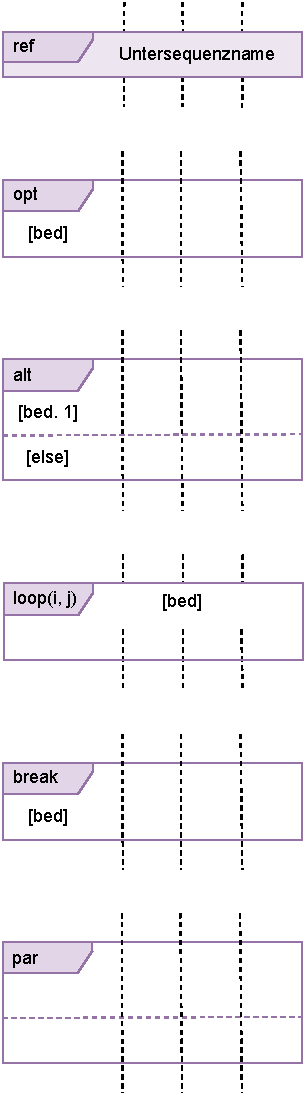
\includegraphics[width=0.2\textwidth]{includes/figures/defi_diagrams_sequenz_operators.pdf}
    \end{wrapfigure}
    %
    Für komplexere Abläufe und bedingte Ausführungsfolgen bietet die UML weitere \emph{Operatoren}\footnote{Sollten die Operatoren in verschiedene Regionen aufgeteilt sein, können diese durch das angeben einer weiteren gestrichelten Linie erweitert werden}:
    \begin{itemize}
        \item \textbf{ref}:

              Leitet verschiedene Lebenslinien in Untersequenzen weiter.
              Dabei muss die Anzahl und Typangabe der referenzierten und eingeführten Lebenslinien übereinstimmen.
        \item \textbf{opt}:

              Ist vergleichbar mit dem \texttt{if}-Statement.
              Führt alle Aktionen in dem Operator aus, wenn die Bedingung \emph{bed} erfüllt ist.
        \item \textbf{alt}:

              Ist vergleichbar mit dem \texttt{switch}-Statement.
              Führt die Aktionen in der ersten Region aus, in der die Bedingung \emph{bed} erfüllt ist.
              Die Bedingungen müssen disjunkt sein.
        \item \textbf{loop}:

              Ist vergleichbar mit dem \texttt{while}-Statement.
              Führt die Aktionen in dem Operator solange aus, bis die Bedingung \emph{bed} verletzt wird.
              Dabei werden mindestens \emph{i} und maximal \emph{j} Iterationen erzwungen.
              \emph{i} und \emph{j} sind optional.
        \item \textbf{break}:

              Ist vergleichbar mit dem \texttt{break}-Statement.
              Springt aus der aktuellen Sequenz, wenn die Bedingung \emph{bed} erfüllt ist.
        \item \textbf{par}:

              Führt alle angegeben Regionen parallel aus.
    \end{itemize}
\end{diag}

\subsection{Zustandsautomaten}

\begin{defi}{Zustandsautomaten}
    \emph{Zustandsautomaten} visualisieren konkrete (interne) Zustände und Ausprägungen mit ihren Übergängen in einem System.
    Sie erweitern Use-Case Diagramme und liefern eine Alternative für Aktivitätsdiagramme.

    Liefern Antwort auf die Frage:
    Wie verhält sich das System in einem bestimmten Zustand bei gewissen Ereignissen?
\end{defi}

\begin{diag}{Zustand (Zustandsautomaten)}
    \begin{wrapfigure}{r}{0.25\textwidth}
        \centering
        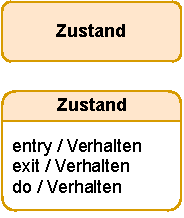
\includegraphics[width=0.2\textwidth]{includes/figures/defi_diagrams_state.pdf}
    \end{wrapfigure}
    Ein \emph{Zustand} beschreibt eine Situation, in der sich das Objekt nicht verändert und ein konstantes Verhalten zeigt.

    Ein Zustand kann ein angegebenes explizites Verhalten besitzen.
    Dieses beschreibt:
    \begin{itemize}
        \item ein Verhalten, welches einmalig beim Eintreten des Zustands ausgeführt wird.
        \item ein Verhalten, welches dauerhaft ausgeführt wird, solange der Zustand aktiv ist.
        \item ein Verhalten, welches einmalig beim Austreten des Zustands ausgeführt wird.
    \end{itemize}
\end{diag}

\begin{diag}{Unterzustände (Zustandsautomaten)}
    Zustände können durch \emph{Unterzustände} erweitert werden:
    \begin{itemize}
        \item Entweder in einen externen Zustand ausgelagert, oder
        \item direkt in einen Zustand hineingezeichnet.
    \end{itemize}

    \begin{center}
        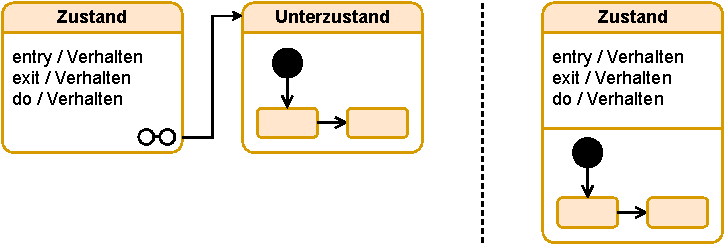
\includegraphics[width=0.5\textwidth]{includes/figures/defi_diagrams_state_substate.pdf}
    \end{center}

    Unterzustände benötigen einen Startzustand oder ausschließlich eindringende Transition.

    Bei der Angabe von mehreren Unterzuständen werden alle parallel ausgeführt.

    Obacht: Wenn eine Transition aus dem Unterzustand den Zustand verlässt, jedoch direkt denselben Unterzustand erneut betritt, wird das \emph{entry} bzw \emph{exit} Verhalten des Zustands ausgeführt.
    Beim Internen Wechsel von Unterzuständen passiert dies nicht.
\end{diag}

\begin{diag}{Transition (Zustandsautomaten)}
    \begin{wrapfigure}{r}{0.25\textwidth}
        \centering
        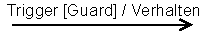
\includegraphics[width=0.2\textwidth]{includes/figures/defi_diagrams_state_transaktion.pdf}
    \end{wrapfigure}
    \emph{Transitionen} bzw. Zustandsübergänge beschreiben Beziehungen zwischen den Einzelzuständen eines Automaten.

    Sie teilen sich in drei Bereiche auf:

    \textbf{Trigger}:
    \begin{itemize}
        \item stoßen eine Transition an
        \item Mehrere Trigger werden durch Kommata getrennt
    \end{itemize}

    \textbf{Guard}:
    \begin{itemize}
        \item Boolsche Bedingung, die entscheidet, ob die Transition tatsächlich durchlaufen wird.
              Ist die Bedingung nicht erfüllt, verfällt der Automat in den Zustand vor der Transition.
    \end{itemize}

    \textbf{Verhalten}:
    \begin{itemize}
        \item Das Verhalten wird beim Durchlaufen der Transition durchgeführt
        \item Vergleichbar mit dem \texttt{entry}-Verhalten von Zuständen
    \end{itemize}
\end{diag}

\begin{diag}{Region}
    \begin{wrapfigure}{r}{0.25\textwidth}
        \centering
        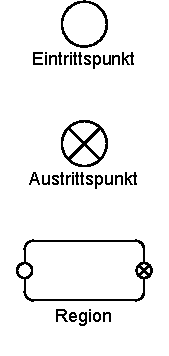
\includegraphics[width=0.2\textwidth]{includes/figures/defi_diagrams_state_region.pdf}
    \end{wrapfigure}
    Um sein Zustandsdiagramm genauer zu strukturieren, kann man einen Teil des Diagramms in einer \emph{Region} zusammenfassen.
    Diese hat \emph{maximal einen} Eintritts- und \emph{maximal einen} Austrittspunkt.

    Der Eintrittspunkt dient für die Region als Startzustand und folgt dementsprechend den selben Regeln\footnote{
        Außer bei Unterzuständen.
        Dort kann dieser Eintrittspunkt ebenfalls \texttt{triggered} sein
    }.

    Der Austrittspunkt dient für die Region als Endzustand und folgt Dementsprechend den selben Regeln.
    Offensichtlich ist jedoch eine ausgehende Kante erlaubt, da man die Region sonst nicht verlassen könnte.

    \vspace{1.5cm}
\end{diag}

\begin{bonus}{Transition in einen Unterzustand (Zustandsautomaten)}
    \begin{wrapfigure}{r}{0.25\textwidth}
        \centering
        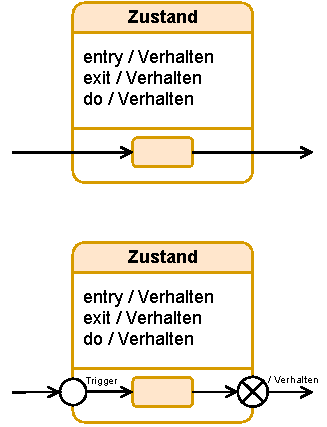
\includegraphics[width=0.25\textwidth]{includes/figures/bonus_diagrams_state_insert.pdf}
    \end{wrapfigure}
    Wenn man in einen bestimmten Unterzustand wechseln möchte, ist es möglich diesen direkt über eine Transition zu erreichen.

    Um eine noch genauere Verwaltung dieses Prozesses zu gewährleisten, kann man erneut \emph{Eintritts-} bzw. \emph{Austritts-Punkte} nutzen.

    Diese blockieren den Objektfluss und benötigen eine externe Freigabe\footnote{Die ausgehenden Transitionen müssen dazu natürlich mit einem Trigger versehen werden}.
    So ist man in dem äußeren Zustand, ohne direkt einen inneren Startzustand wählen zu müssen (innerer Pseudozustand).

    \emph{Austrittspunkte} können weiterhin genutzt werden, um gebündelt den ganzen Zustand zu verlassen.
    Wenn man - vor allem bei parallelen Unterzuständen - einfache Kanten nach außen legt, kann es passieren, dass man sich gleichzeitig innerhalb und außerhalb von einem Zustand befindet.
    Dies kann man verhindern, indem man von dem Austrittspunkt ein Event auslöst, welche alle inneren Zustände verlässt:

    \begin{center}
        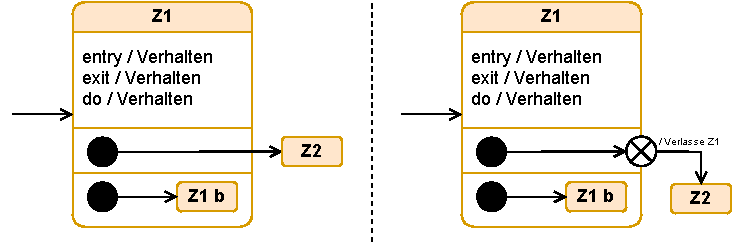
\includegraphics[width=0.75\textwidth]{includes/figures/bonus_diagrams_state_exit.pdf}
    \end{center}
    Wenn man den linken Zustand \emph{Z1} betritt, befindet man sich gleichzeitig in \emph{Z2} und \emph{Z1 b}\footnote{also auch \emph{Z1}}.
    Rechts verhindert der Austrittspunkt dies.
\end{bonus}

\begin{diag}{Kontrollelemente zur Ablaufsteuerung (Zustandsautomaten)}
    \begin{wrapfigure}{r}{0.25\textwidth}
        \centering
        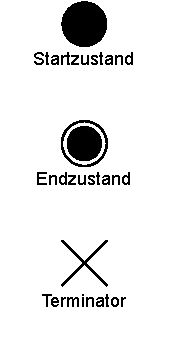
\includegraphics[width=0.15\textwidth]{includes/figures/defi_diagrams_state_start.pdf}
    \end{wrapfigure}
    Zu den Kontrollelementen zählen sogenannte \emph{Pseudozustände}.
    Diese haben keinerlei inhaltlichen Nutzen, sind also keine wirklichen Zustände.
    Trotzdem werden diese zur Ablaufsteuerung gebraucht.

    \textbf{Startzustand} bzw. initial pseudostate:
    \begin{itemize}
        \item vergleichbar mit Startknoten aus dem Aktivitätsdiagramm
        \item Eindeutigkeit: verweist auf \emph{genau einen} Zielzustand
        \item Untriggered: darf keine Bedingung beinhalten
        \item keine eingehende Transition erlaubt
        \item Global eindeutig: \emph{maximal ein} Startzustand pro Region
    \end{itemize}

    \textbf{Endzustand} bzw. final pseudostate
    \begin{itemize}
        \item vergleichbar mit Endknoten aus dem Aktivitätsdiagramm
        \item Beendet den gesamten Zustandsautomaten
        \item Keine ausgehende Transition erlaubt
        \item Global eindeutig: \emph{Genau einen} Endzustand pro Diagramm erlaubt
    \end{itemize}

    \textbf{Terminator}
    \begin{itemize}
        \item Vergleichbar mit der Objektzerstörung in Sequenzdiagrammen
        \item erweitert den Endzustand
        \item löscht bzw. zerstört zusätzlich das gesamte Objekt
        \item wird in der Regel verwendet, wenn due Objekte dynamisch erstellt / gelöscht werden
    \end{itemize}
\end{diag}

\begin{diag}{Kontrollelemente zur Ablaufsteuerung zur Strukturierung (Zustandsautomaten)}
    \begin{wrapfigure}{r}{0.25\textwidth}
        \centering
        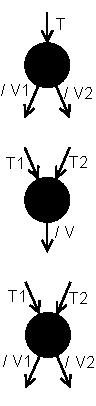
\includegraphics[width=0.1\textwidth]{includes/figures/defi_diagrams_state_crosspoint.pdf}
    \end{wrapfigure}
    \emph{Kreuzungspunkte} vereinfachen Transitionspfade, indem sie gemeinsame Teile bündeln.

    Man unterscheidet in drei Verarbeitungsarten:
    \begin{itemize}
        \item \textbf{Vereinigung von Triggern}:

              Wenn aus einem Zustand mehrere Transitionen ausgehen, welche mit dem selben Trigger versehen sind, kann man eine Ausgehende Transition mit diesem Trigger erstellen, welche in einen Kreuzungspunkt führt.
              Aus diesem gehen die verschiedenen Transitionen mit deren unterschiedlichen Verhalten aus.
        \item \textbf{Vereinigung von Bedingungen \& Verhalten}

              Wenn aus zwei unterschiedlichen Zuständen das selbe Verhalten ausgeht, kann dies kombiniert werden.
              Die Trigger sind dabei offensichtlich unterschiedlich.
        \item \textbf{Kombination aus beiden}
    \end{itemize}

    Die Guards der ausgehenden Transitionen müssen dabei jedoch nicht disjunkt sein.
\end{diag}

\begin{diag}{Kontrollelemente zur Ablaufsteuerung für Bedingungen (Zustandsautomaten)}
    \begin{wrapfigure}{r}{0.25\textwidth}
        \centering
        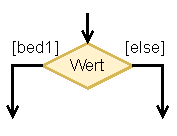
\includegraphics[width=0.2\textwidth]{includes/figures/defi_diagrams_state_if.pdf}
    \end{wrapfigure}
    \emph{Entscheidungsknoten} entsprechen dem \texttt{switch}-Statement.
    Die Variable bzw. das Entscheidungskriterium wird in die Raute gezeichnet.
    Die Bedingungen werden dann in die Guards der ausgehenden Kanten geschrieben.
    Dabei kann ebenfalls eine wertunabhängige Abfrage genutzt werden (z.B. else, true etc.).

    Alle Bedingungen müssen disjunkt sein und es muss zu jeder Zeit des Programms der gesamte Wertebereich durch die Bedingungen abgedeckt sein.
    Es muss also jederzeit möglich sein den Zustand vor dem Entscheidungsknoten zu verlassen und den Entscheidungsknoten zu passieren.
\end{diag}

\begin{bonus}{Unterschiede von Entscheidungsknoten und Kreuzungspunkten (Zustandsautomaten)}
    Im Gegensatz zu Kreuzungspunkten wird jedoch zuerst das Verhalten der eingehenden Kante ausgeführt, danach die Bedingungen getestet.

    \begin{center}
        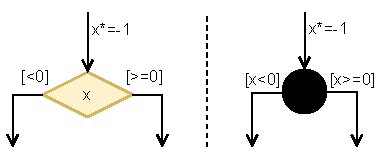
\includegraphics[width=0.5\textwidth]{includes/figures/bonus_diagrams_state_if.pdf}
    \end{center}

    Wenn man nun in diese Beiden Objekte die Variable \texttt{int x = 1} einführt, unterscheidet sich der Ablauf der Bearbeitung:
    \begin{itemize}
        \item \textbf{Entscheidungsknoten}:

              \begin{tabular}{lll}
                  1. & \texttt{int x = 1}                       & | x = 1                   \\
                  2. & \texttt{x *= -1}                         & | x = -1                  \\
                  3. & \texttt{x < 0}                           & | true                    \\
                     & \textcolor{gray}{\texttt{x >= 0}}        & \textcolor{gray}{| false} \\
                  4. & verfolge die linke Transition mit x = -1 &
              \end{tabular}
        \item \textbf{Kreuzungspunkt}:

              \begin{tabular}{lll}
                  1. & \texttt{int x = 1}                        & | x = 1  \\
                  2. & \texttt{x < 0}                            & | false  \\
                  3. & \texttt{x >= 0}                           & | true   \\
                  4. & \texttt{x *= 1}                           & | x = -1 \\
                  5. & verfolge die rechte Transition mit x = -1 &
              \end{tabular}
    \end{itemize}
\end{bonus}

\begin{diag}{Kontrollelemente zur Ablaufsteuerung zur Parallelisierung (Zustandsautomaten)}
    \begin{wrapfigure}{r}{0.25\textwidth}
        \centering
        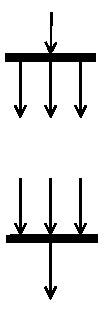
\includegraphics[width=0.1\textwidth]{includes/figures/defi_diagrams_state_parallel.pdf}
    \end{wrapfigure}
    Wie bei Aktivitätsdiagrammen kann man ebenfalls bei Zustandsautomaten \emph{parallele Zweige} erstellen.

    Jeder Parallelzweig muss immer in einem eindeutigen Zustand sein.
    Dementsprechend sind Pseudozustände nicht erlaubt.

    Bei Unterzuständen kann man die Trennlinie weglassen.
    Dort wird jede Region automatisch parallel gestartet.

    Wenn man jedoch auf einer Ebene Parallelitäten erstellen möchte, muss man Trennlinien und Joins benutzen.

    \vspace{0.5cm}
\end{diag}

\begin{diag}{Historie (Zustandsautomaten)}
    \begin{wrapfigure}{r}{0.25\textwidth}
        \centering
        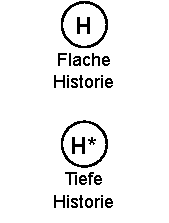
\includegraphics[width=0.2\textwidth]{includes/figures/defi_diagrams_state_history.pdf}
    \end{wrapfigure}
    Wenn man Zustände speichern möchte, muss man eine \emph{Historie} anlegen.

    \begin{itemize}
        \item Bei Verlassen eines Zustands wird sich der letzte Aktive Unterzustand gemerkt.
        \item Beim erneuten Betreten dieses Zustands wird der gemerkte Unterzustand betreten.
        \item Sollte kein Zustand gespeichert sein, wird der default Startzustand betreten.
        \item Dabei darf maximal ein Historienelement pro Zustand auf gleicher Ebene existieren.
        \item Jedoch ist es natürlich möglich einen Zustand über hierarchische Strukturen mehrfach zu speichern.
        \item Beim Erreichen eines beliebigen Endzustands wird die gesamte Historie gelöscht.
    \end{itemize}

    \texttt{H} speichert nur den Zustand der gleichen Ebene.
    Im Gegensatz dazu speichert \texttt{H*} rekursiv ebenfalls Unterzustände. Dies ist vergleichbar mit \texttt{copy()} bzw \texttt{deepcopy()} von Arrays.
\end{diag}

\begin{example}{Historie (Zustandsautomaten)}
    \begin{center}
        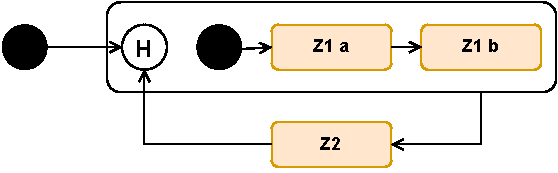
\includegraphics[width=0.5\textwidth]{includes/figures/example_diagrams_state_history.pdf}
    \end{center}

    \begin{enumerate}
        \item In diesem Beispiel wird nach dem Startknoten direkt die Region um \emph{Z1} betreten.
        \item  Da \emph{H} keinen Zustand gespeichert hat, wird der Startknoten in der Region genutzt.
        \item \emph{Z1 a} wird betreten.
        \item \emph{Z1 b} wird betreten.
        \item Die Region wird verlassen und \emph{H} speichert \emph{Z1 b}.
              Wir befinden uns in \emph{Z2}
        \item Beim erneuten Betreten der Region wird der gespeicherte Zustand \emph{Z1 b} betreten
        \item Also ist es in diesem expliziten Beispiel nicht möglich, \emph{Z1 a} erneut zu betreten.
    \end{enumerate}
\end{example}